\documentclass[11pt]{article}

\usepackage[margin=1in]{geometry}
\usepackage{amsmath,amssymb,amsthm}
\usepackage{algorithm}
\usepackage{algpseudocode}
\usepackage{booktabs}
\usepackage{hyperref}
\usepackage{xcolor}
\usepackage{tikz}
\usetikzlibrary{positioning,calc,arrows.meta}

\newtheorem{theorem}{Theorem}
\newtheorem{lemma}[theorem]{Lemma}
\newtheorem{definition}[theorem]{Definition}
\newtheorem{corollary}[theorem]{Corollary}

\newcommand{\hash}{\mathcal{H}}
\newcommand{\prf}{\mathrm{PRF}}
\newcommand{\adv}{\mathbf{Adv}}
\newcommand{\secpar}{\lambda}
\newcommand{\bin}{\{0,1\}}
\newcommand{\concat}{\,\|\,}

\title{PUP: Post-quantum Unicity Protocol\\[6pt]
\large Nonce-Bound Hash-Based Signatures for Blockchains}

\author{Tal Zisckind\\[4pt]\normalsize Rhombus Tech}

\date{June 2026}

\begin{document}

\maketitle

\begin{abstract}
The entire complexity of SLH-DSA (SPHINCS+)---its hypertree, FORS
few-time signatures, and $7{,}856$-byte outputs---exists to solve one
problem: preventing leaf reuse without trusting the signer's state.
We observe that account-based blockchains already solve this problem.
Every such chain enforces a sequential per-account nonce, providing
exactly the monotonic, gap-free index that stateful Merkle-tree
signature schemes require.

PUP (Post-quantum Unicity Protocol) exploits this
observation to replace SPHINCS+'s stateless machinery with a single
Merkle tree of W-OTS+ leaves, where the leaf index \emph{is} the
transaction nonce. The on-chain verifier caches the current
authentication path; the signer sends only the siblings that change
between consecutive leaves---an average of one hash per signature.
Because the blockchain state fixes the adversary's target leaf
deterministically, the EU-CMA-to-OTS security reduction is tight,
eliminating the $2^{h/d}$ reduction loss inherent in SPHINCS+'s
hypertree simulator.

At the recommended parameter set ($n = 20$), the result is
${\sim}884$-byte average signatures ($8.9\times$ smaller than
SPHINCS+-128s), ${\sim}6\times$ faster verification, and a tighter
security proof, all under hash-only assumptions at ${\sim}2^{71}$
quantum security. A compact parameter set ($n = 16$) achieves
${\sim}580$-byte signatures ($13.5\times$ smaller) at ${\sim}2^{55}$
quantum security. We provide a reference implementation with tests
covering correctness, rejection, and operational safety.
\end{abstract}

\section{Introduction}

The post-quantum migration of blockchain signature schemes presents a
fundamental tension. Hash-based signatures offer security under minimal
assumptions---preimage and collision resistance of the underlying hash
function---but the NIST-standardized stateless scheme SLH-DSA
(SPHINCS+)~\cite{sphincs} produces signatures of $7{,}856$ bytes at the
128-bit security level. For blockchains, where every signature is
propagated to all nodes and stored permanently, this $122\times$ blowup
over ECDSA is a serious throughput constraint.

Stateful hash-based schemes (XMSS~\cite{xmss}, LMS~\cite{lms}) produce
much smaller signatures (${\sim}2{,}500$ bytes) but carry a catastrophic
failure mode: if a one-time signing key is used twice, the scheme is
completely broken. NIST SP 800-208~\cite{nist-sp800-208} explicitly
warns that ``the consequences of a one-time signature key being reused
can be dire'' and recommends against deployment without rigorous state
management guarantees.

This state management problem---tracking which leaf has been used and
ensuring no leaf is ever reused across crashes, backups, and operational
errors---is precisely what drove the development of stateless schemes
like SPHINCS+. The entire hypertree construction, the FORS few-time
signature layer, and the resulting signature size exist to avoid trusting
the signer's state.

\paragraph{Observation.} Blockchains already solve this problem.
Every account-based blockchain maintains a per-account nonce: a
sequential counter that is incremented with each transaction and
enforced by consensus. A transaction with nonce $i$ is accepted if and
only if the account's current nonce is $i$. This is precisely the
sequential leaf-usage guarantee that stateful hash-based signatures
require. The nonce is not a heuristic or an application-layer
convention---it is enforced by consensus, crash-safe by design, and
replicated across every node. It provides strictly stronger guarantees
than any local state file a signer could maintain.

This observation implies that, for account-based blockchains, the
complexity of SPHINCS+ is \emph{unnecessary}: the hypertree exists to
tolerate arbitrary-order leaf access, but nonces enforce sequential
access; FORS exists to tolerate bounded leaf reuse, but nonces prevent
any reuse; the large signature exists to carry a full authentication
path, but the chain can cache the path between transactions. Removing
all three components yields a flat Merkle tree of one-time signatures
with dramatically smaller signatures, faster verification, and a
tighter security proof.

\paragraph{Distinction from XMSS/LMS.}
At the structural level, PUP uses the same primitives as XMSS: a
Merkle tree over W-OTS+ leaves. The novelty is \emph{not} the
primitives but the three techniques that become possible once the
blockchain is treated as a co-signer rather than a passive verifier:

\begin{enumerate}
\item \textbf{Nonce--leaf binding (Section~\ref{sec:construction}).}
XMSS and LMS require the signer to maintain a persistent, crash-safe
counter and never reuse a leaf---the failure mode that motivated
SPHINCS+'s statelessness. PUP binds the leaf index to the transaction
nonce, a counter that the blockchain already maintains and enforces at
the consensus layer. The signer derives the correct leaf from the nonce
it must already know to construct a valid transaction, eliminating the
operational risk \emph{by construction} rather than by discipline.
No prior scheme makes this binding.

\item \textbf{Delta-compressed authentication paths
(Section~\ref{sec:delta}).}
XMSS signatures carry a full authentication path ($H \cdot n$ bytes)
with every signature. PUP caches the current authentication path
on-chain and transmits only the siblings that change between
consecutive leaves. We prove (Theorem~\ref{thm:avg-delta}) that the
expected delta is exactly one hash per signature, reducing the
per-signature authentication overhead from $H \cdot n = 320$ bytes to
$n = 16$ bytes on average---a $20\times$ compression of the path
component alone. This technique is novel; it does not appear in XMSS,
LMS, SPHINCS+, BPQS, or SHRINCS.

\item \textbf{Tight security reduction (Section~\ref{sec:security}).}
In XMSS, the EU-CMA-to-OTS reduction loses a factor of $2^H$ because
the simulator must guess which of $2^H$ leaves the adversary will
target. SPHINCS+ reduces this to $2^{h/d}$ via its hypertree structure
but does not eliminate it. Because the blockchain state fixes the
adversary's target leaf to $\mathsf{next\_index}$ (deterministically
equal to the number of prior signing queries), PUP's reduction embeds
its challenge at the known target leaf with probability~$1$, yielding a
\emph{tight} reduction with no guessing loss. This tightness is a
direct consequence of nonce--leaf binding and does not hold for any
scheme where the target leaf is adversarially chosen.
\end{enumerate}

The combined effect at the recommended parameters ($n = 20$) is
${\sim}884$-byte average signatures (worst case $1{,}244$ bytes),
${\sim}6\times$ faster verification than SPHINCS+-128s, ${\sim}2^{71}$
quantum security, and a tighter security proof, all under the same
hash-only assumption. A compact parameter set ($n = 16$) further
reduces signatures to ${\sim}580$ bytes at ${\sim}2^{55}$ quantum
security, comparable to SPHINCS+-128s.
Figure~\ref{fig:structure} summarizes the structural simplification.

\begin{figure}[t]
\centering
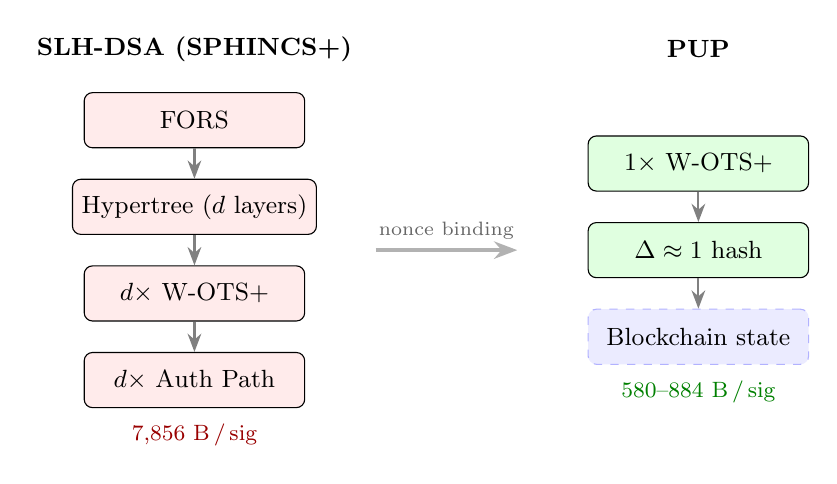
\begin{tikzpicture}[
  box/.style={draw, rounded corners=3pt, minimum width=28mm,
    minimum height=7mm, font=\small, align=center},
  lbl/.style={font=\footnotesize, align=center},
  arr/.style={-{Stealth}, thick, black!50},
  xscale=1
]
% ---- SPHINCS+ (left) ----
\node[font=\small\bfseries] at (-3.2,4.2) {SLH-DSA (SPHINCS+)};

\node[box, fill=red!8] (fors) at (-3.2,3.3) {FORS};
\node[box, fill=red!8] (ht) at (-3.2,2.2)
  {Hypertree ($d$ layers)};
\node[box, fill=red!8] (otsx) at (-3.2,1.1)
  {$d \times$ W-OTS+};
\node[box, fill=red!8] (authx) at (-3.2,0.0)
  {$d \times$ Auth Path};

\draw[arr] (fors) -- (ht);
\draw[arr] (ht) -- (otsx);
\draw[arr] (otsx) -- (authx);

\node[lbl, red!60!black] at (-3.2,-0.7)
  {$7{,}856$ B\,/\,sig};

% ---- Arrow ----
\draw[-{Stealth}, very thick, black!30]
  (-0.9,1.65) -- node[above, font=\scriptsize, black!60]
  {nonce binding} (0.9,1.65);

% ---- PUP (right) ----
\node[font=\small\bfseries] at (3.2,4.2) {PUP};

\node[box, fill=green!12] (ots) at (3.2,2.75)
  {$1 \times$ W-OTS+};
\node[box, fill=green!12] (delt) at (3.2,1.65)
  {$\Delta \approx 1$ hash};
\node[box, fill=blue!8, draw=blue!30, dashed] (chain)
  at (3.2,0.55) {Blockchain state};

\draw[arr] (ots) -- (delt);
\draw[arr] (delt) -- (chain);

\node[lbl, green!50!black] at (3.2,-0.15)
  {$580$--$884$ B\,/\,sig};
\end{tikzpicture}
\caption{Structural comparison.  SPHINCS+ uses a $d$-level hypertree,
FORS few-time signatures, and $d$ full authentication paths to achieve
statelessness.  PUP replaces all three with a single W-OTS+ signature
and a delta of ${\approx}\,1$ hash, by binding leaf indices to
blockchain-enforced nonces and caching the authentication path
on-chain.}\label{fig:structure}
\end{figure}

\section{Preliminaries}

\subsection{Notation}

We write $[n]$ for $\{0, \ldots, n-1\}$. For an integer $i > 0$,
$\nu_2(i)$ denotes the 2-adic valuation (the largest $k$ such that
$2^k \mid i$). We define $\nu_2(0) = 0$ by convention; this value is
never used in the scheme (delta transitions start at $i = 1$). All hash functions output $n$
bytes. $\concat$ denotes concatenation.

\subsection{Tweaked Hash Function}

Following SPHINCS+~\cite{sphincs}, every hash invocation is bound to a
unique address to prevent multi-target attacks.

\begin{definition}[Tweaked Hash]
Let $\hash : \bin^* \to \bin^{8n}$ be a hash function (instantiated as
SHA-256 truncated to $n$ bytes). For a public seed
$\mathsf{seed} \in \bin^{8n}$, domain separator $d \in \bin^8$, and
address $\mathsf{addr} \in \bin^*$, define:
\[
\hash_n^d(\mathsf{seed}, \mathsf{addr}, x) = \hash(d \concat
\mathsf{seed} \concat \mathsf{addr} \concat x)[{:}n]
\]
Each key pair generates an independent $\mathsf{seed}$, ensuring that
different key pairs evaluate independent tweaked-hash families in the
random oracle model and preventing multi-target attacks across accounts.
\end{definition}

We use four domain separators for the tweaked hash:
$\mathsf{LEAF} = \mathtt{0x00}$,
$\mathsf{NODE} = \mathtt{0x01}$, $\mathsf{CHAIN} = \mathtt{0x02}$,
$\mathsf{MSG} = \mathtt{0x03}$.
A separate PRF derives per-leaf secret keys:
$\prf(\mathsf{sk}, i) = \mathrm{HMAC}\text{-}\mathrm{SHA256}(\mathsf{sk}, i)[{:}n]$.

Address structures ensure that every hash call site receives a unique
tweak. In all cases, $\mathsf{seed}$ is prepended via the tweaked-hash
definition above; only the variable address components are listed:
\begin{itemize}
\item Chain hash: $\mathsf{addr} = (\mathsf{leaf\_idx} \concat
\mathsf{chain\_idx} \concat \mathsf{step})$
\item Leaf hash: $\mathsf{addr} = (\mathsf{leaf\_idx})$
\item Node hash: $\mathsf{addr} = (\mathsf{level} \concat
\mathsf{index})$
\end{itemize}

\subsection{W-OTS+ (Winternitz One-Time Signatures)}

We use W-OTS+~\cite{wots} with Winternitz parameter $w$. A message $m$
is hashed to $n$ bytes via
$\hash_n^{\mathsf{MSG}}(\mathsf{leaf\_idx},\, m)$, then encoded as
$\ell_1 = \lceil 8n / \lg w
\rceil$ base-$w$ digits. A checksum of $\ell_2 = \lceil \lceil
\log_2(\ell_1(w-1) + 1) \rceil / \lg w \rceil$ digits is appended,
giving $\ell = \ell_1 + \ell_2$ total digits.

Each digit $d_i \in [w]$ indexes into a hash chain of length $w$:
\[
c_i^{(j)} = \hash_n^{\mathsf{CHAIN}}(\mathsf{addr}(i, j),\, c_i^{(j-1)})
\quad\text{for } j \in [1, w)
\]
where $c_i^{(0)} = \mathsf{sk}_i$ is the secret chain seed.

The signature reveals $\sigma_i = c_i^{(d_i)}$. Verification computes
$c_i^{(w-1)}$ from $\sigma_i$ by iterating $w - 1 - d_i$ more steps
and checks equality with the public chain endpoint $\mathsf{pk}_i$.

The checksum ensures that for any two distinct messages, at least one
digit \emph{decreases}, requiring backward iteration (hash inversion)
to forge.

\subsection{Merkle Trees}

A binary Merkle tree of height $H$ over $2^H$ leaves uses the tweaked
internal hash:
\[
\mathsf{node}(\ell, r, \mathsf{lv}, \mathsf{idx}) =
\hash_n^{\mathsf{NODE}}((\mathsf{lv} \concat \mathsf{idx}),\, \ell \concat r)
\]

The authentication path for leaf $i$ consists of the $H$ sibling nodes
along the path from leaf $i$ to the root.

\subsection{Blockchain State Model}

We require an execution environment that provides the following
guarantees, which we collectively call the \emph{sequential nonce
model}:

\begin{definition}[Sequential Nonce Model]\label{def:nonce}
An account-based blockchain maintains, for each account $A$, a nonce
$A.\mathsf{nonce} \in \mathbb{N}$ initialized to $0$. A transaction
from $A$ carrying nonce $i$ is valid if and only if
$A.\mathsf{nonce} = i$. Upon inclusion in a finalized block, the chain
sets $A.\mathsf{nonce} \leftarrow i + 1$. The model provides three
guarantees:
\begin{enumerate}
\item \textbf{Monotonicity.} The nonce is strictly increasing:
transactions from $A$ are processed in nonce order $0, 1, 2, \ldots$
\item \textbf{Gap-freedom.} No nonce value is skipped. A transaction
with nonce $i + 1$ cannot be included until a transaction with nonce
$i$ has been finalized.
\item \textbf{Consensus enforcement.} These properties are enforced by
every validating node, not by the signer. A signer that attempts to
reuse or skip a nonce produces an invalid transaction that is rejected
by the network.
\end{enumerate}
\end{definition}

This model captures Ethereum (EIP-155~\cite{eip155}), Aptos, and any
account-based blockchain with sequential per-account nonces. Chains
that use alternative replay protection (e.g., Solana's recent
blockhashes, Sui's object versioning) do not satisfy this model without
protocol adaptation. UTXO-based chains (Bitcoin) do not have
per-account nonces and are outside our scope.

The sequential nonce model provides strictly stronger guarantees than
the state management required by XMSS or LMS: those schemes need
only that the signer never reuse a leaf, while the nonce model
guarantees sequential, gap-free usage enforced by consensus across all
nodes. This surplus of structure is what enables delta compression
(Section~\ref{sec:delta}).

\section{Construction}\label{sec:construction}

\subsection{Parameters}

\begin{center}
\begin{tabular}{lll}
\toprule
Parameter & Default & Description \\
\midrule
$n$ & 16 & Hash output bytes \\
$w$ & 16 & Winternitz parameter \\
$H$ & 20 & Tree height ($2^H$ max signatures) \\
$\ell$ & 35 & W-OTS+ chains ($\ell_1 = 32$, $\ell_2 = 3$) \\
\bottomrule
\end{tabular}
\end{center}

\paragraph{Recommended parameters.}
We present derivations using $n = 16$ for concreteness (smaller
numbers, easier to follow). However, we recommend $n = 20$ for
deployment. At $n = 20$, $\ell_1 = 40$, $\ell_2 = 3$, $\ell = 43$,
yielding $884$-byte average signatures with ${\sim}2^{71}$ quantum
security---a substantial margin over the ${\sim}2^{55}$ level at
$n = 16$. The $n = 16$ parameter set remains useful for
throughput-constrained chains where the ${\sim}55$-bit quantum security
(comparable to SPHINCS+-128s) is acceptable and the $34\%$ signature
reduction matters. Section~\ref{sec:security} provides concrete bounds
for both parameter sets.

\subsection{Key Generation}

Given a random seed $\mathsf{sk} \xleftarrow{\$} \bin^{256}$ and a
random public seed $\mathsf{seed} \xleftarrow{\$} \bin^{8n}$:

\begin{enumerate}
\item For each $i \in [2^H]$, derive the $i$-th W-OTS+ key pair
$(\mathsf{sk}_i, \mathsf{pk}_i)$ using $\prf(\mathsf{sk}, i)$.
\item Compute leaf hashes:
$L_i = \hash_n^{\mathsf{LEAF}}(\mathsf{seed},\, i,\,
\mathsf{pk}_i^{(0)} \concat \cdots \concat
\mathsf{pk}_i^{(\ell-1)})$.
\item Build the Merkle tree over $\{L_i\}$ using
$\hash_n^{\mathsf{NODE}}(\mathsf{seed},\, \cdot)$.  The root $R$ is
the verification key.
\end{enumerate}

The full signing key is $\mathsf{SK} = (\mathsf{sk}, \mathsf{seed},
\text{tree})$. The public key is $\mathsf{PK} = (R, \mathsf{seed})$.

\subsection{Account Registration}

To register on-chain, the signer provides:
\begin{itemize}
\item The leaf hash $L_0$
\item The authentication path $\mathsf{auth}_0$ for leaf $0$
\end{itemize}

The chain verifies that $L_0$ and $\mathsf{auth}_0$ resolve to the
public root $R$, then stores:
\[
\mathsf{state} = (\mathsf{next\_index} = 0,\; \mathsf{cached} =
\mathsf{auth}_0)
\]

This costs $H \cdot n + 4$ bytes per account (324 bytes at default
parameters): $H \cdot n$ bytes for the cached siblings plus $4$ bytes
for the 32-bit next-index counter.

\subsection{Signing}

To sign message $m$ at index $i = \mathsf{state.next\_index}$:

\begin{enumerate}
\item Compute the delta $\Delta$: the sibling hashes that differ between
$\mathsf{auth}_i$ and $\mathsf{auth}_{i+1}$, excluding the one
derivable by the verifier (see Section~\ref{sec:delta}).
\item Form the \emph{bound payload}
$\hat{m} = \mathsf{LE64}(|m|) \concat m \concat \Delta[0] \concat
\cdots \concat \Delta[|\Delta|-1]$, where $\mathsf{LE64}$ encodes the
message length as an 8-byte little-endian integer.
\item Compute the W-OTS+ signature $\sigma_{\mathsf{ots}}$ on $\hat{m}$
using the key at leaf $i$.
\end{enumerate}

The delta is computed \emph{before} signing so that the OTS signature
covers both the message and the authentication-path update. This
prevents a block proposer from tampering with $\Delta$ in transit: any
modification invalidates $\sigma_{\mathsf{ots}}$.

The signature is $\Sigma = (i, \sigma_{\mathsf{ots}}, \Delta)$.

\subsection{Verification and State Update}

Given public key $\mathsf{PK} = (R, \mathsf{seed})$, message $m$,
signature $\Sigma = (i, \sigma_{\mathsf{ots}}, \Delta)$, and on-chain
state $\mathsf{state}$:

\begin{enumerate}
\item \textbf{Index check:} Reject if $i \neq
\mathsf{state.next\_index}$.
\item \textbf{Bind payload:} Reconstruct
$\hat{m} = \mathsf{LE64}(|m|) \concat m \concat \Delta[0] \concat
\cdots \concat \Delta[|\Delta|-1]$.
\item \textbf{OTS recovery:} Compute the leaf hash $L$ from
$\sigma_{\mathsf{ots}}$ and $\hat{m}$ by completing each W-OTS+ chain
to position $w - 1$ and hashing the concatenated endpoints.
\item \textbf{Root check:} Walk from $L$ up the Merkle tree using
$\mathsf{state.cached}$ as the sibling hashes. Reject if the computed
root $\neq R$.
\item \textbf{State update:} If $i + 1 = 2^H$, the key is exhausted;
set $\mathsf{state.next\_index} \leftarrow 2^H$ and skip the sibling
update. Otherwise, compute the new cached siblings for leaf $i + 1$:
\begin{itemize}
\item Let $M = \nu_2(i+1) + 1$ (the \emph{merge level}).
\item Levels $\geq M$: unchanged (leaves $i$ and $i+1$ share these
siblings).
\item Level $M - 1$: \emph{derived} by the verifier---walk up $M - 1$
levels from $L$ using the old cached siblings.
\item Levels $0, \ldots, M - 2$: taken from $\Delta$.
\end{itemize}
\item Set $\mathsf{state.next\_index} \leftarrow i + 1$.
\end{enumerate}

\subsection{Formal Specification}

Algorithms~\ref{alg:keygen}--\ref{alg:verify} give the complete
specification. $\mathsf{WOTS.KG}$ generates a W-OTS+ key pair from a
seed, $\mathsf{WOTS.Sign}$ produces a one-time signature, and
$\mathsf{WOTS.PkRecover}$ recovers the leaf hash from a signature and
message by completing each chain and hashing the endpoints.
$\mathsf{MerkleRoot}$ walks from a leaf hash to the root using
the provided siblings. $\mathsf{WalkUp}$ hashes upward through
$k$ levels of siblings from a starting value.

\begin{algorithm}[t]
\caption{$\mathsf{PUP.KeyGen}(1^\secpar)$}\label{alg:keygen}
\begin{algorithmic}[1]
\State $\mathsf{sk} \xleftarrow{\$} \bin^{256}$;\quad
$\mathsf{seed} \xleftarrow{\$} \bin^{8n}$
\For{$i = 0$ \textbf{to} $2^H - 1$}
  \State $(\mathsf{sk}_i, \mathsf{pk}_i) \gets
  \mathsf{WOTS.KG}(\prf(\mathsf{sk}, i),\, \mathsf{seed},\, i)$
  \State $L_i \gets \hash_n^{\mathsf{LEAF}}(\mathsf{seed},\, i,\,
  \mathsf{pk}_i)$
\EndFor
\State $\mathsf{tree} \gets \mathsf{BuildMerkle}(\{L_i\},\,
\mathsf{seed})$;\quad $R \gets \mathsf{tree.root}$
\State \Return $\mathsf{SK} = (\mathsf{sk}, \mathsf{seed},
\mathsf{tree})$,\; $\mathsf{PK} = (R, \mathsf{seed})$
\end{algorithmic}
\end{algorithm}

\begin{algorithm}[t]
\caption{$\mathsf{PUP.Sign}(\mathsf{SK},\, m,\, i)$
\hfill \textit{// $i = \mathsf{state.next\_index}$}}
\label{alg:sign}
\begin{algorithmic}[1]
\State $(\mathsf{sk}_i, \_) \gets \mathsf{WOTS.KG}(\prf(\mathsf{SK.sk},
i),\, \mathsf{SK.seed},\, i)$
\If{$i + 1 < 2^H$}
  \State $M \gets \nu_2(i + 1) + 1$
  \State $\Delta \gets
  (\mathsf{SK.tree.sibling}(i{+}1, 0),\, \ldots,\,
  \mathsf{SK.tree.sibling}(i{+}1, M{-}2))$
\Else\ $\Delta \gets ()$
\EndIf
\State $\hat{m} \gets \mathsf{LE64}(|m|) \concat m \concat
\Delta[0] \concat \cdots \concat \Delta[|\Delta|{-}1]$
\State $\sigma_{\mathsf{ots}} \gets \mathsf{WOTS.Sign}(\mathsf{sk}_i,
\, \mathsf{SK.seed},\, i,\, \hat{m})$
\State \Return $\Sigma = (i,\, \sigma_{\mathsf{ots}},\, \Delta)$
\end{algorithmic}
\end{algorithm}

\begin{algorithm}[t]
\caption{$\mathsf{PUP.Verify}(\mathsf{PK},\, m,\, \Sigma,\,
\mathsf{state})$}\label{alg:verify}
\begin{algorithmic}[1]
\State Parse $\Sigma = (i,\, \sigma_{\mathsf{ots}},\, \Delta)$
\If{$i \neq \mathsf{state.next\_index}$}
  \Return $(\bot,\, \mathsf{state})$
\EndIf
\State $\hat{m} \gets \mathsf{LE64}(|m|) \concat m \concat
\Delta[0] \concat \cdots \concat \Delta[|\Delta|{-}1]$
\State $L \gets \mathsf{WOTS.PkRecover}(\sigma_{\mathsf{ots}},\,
\mathsf{PK.seed},\, i,\, \hat{m})$
\State $R' \gets \mathsf{MerkleRoot}(L,\, \mathsf{state.cached},\, i)$
\If{$R' \neq \mathsf{PK.}R$}
  \Return $(\bot,\, \mathsf{state})$
\EndIf
\If{$i + 1 = 2^H$}
  \Return $(\top,\; (\mathsf{next\_index}{=}2^H,\,
  \mathsf{cached}{=}\mathsf{state.cached}))$
\EndIf
\State $M \gets \nu_2(i + 1) + 1$
\State $\mathsf{derived} \gets \mathsf{WalkUp}(L,\,
\mathsf{state.cached}[0{:}M{-}2],\, i)$
\State $\mathsf{cached}' \gets \mathsf{state.cached}$
\State $\mathsf{cached}'[M{-}1] \gets \mathsf{derived}$
\For{$k = 0$ \textbf{to} $M - 2$}
  \State $\mathsf{cached}'[k] \gets \Delta[k]$
\EndFor
\State \Return $(\top,\; (\mathsf{next\_index}{=}i{+}1,\,
\mathsf{cached}{=}\mathsf{cached}'))$
\end{algorithmic}
\end{algorithm}

\section{Delta Compression}\label{sec:delta}

\subsection{Merge Level}

\begin{definition}
For $i > 0$, the \emph{merge level} is $M(i) = \nu_2(i) + 1$. This is
the lowest Merkle tree level at which leaf $i - 1$ and leaf $i$ share a
common ancestor \emph{not} shared by the previous sibling pair.
\end{definition}

\begin{lemma}\label{lem:changed}
The number of authentication path siblings that differ between leaf
$i - 1$ and leaf $i$ is exactly $M(i)$.
\end{lemma}

\begin{proof}
Leaves $i - 1$ and $i$ are consecutive. At level $0$, they have
different siblings (trivially). At level $k < M(i)$, the subtree index
$\lfloor (i-1) / 2^k \rfloor \neq \lfloor i / 2^k \rfloor$, so the
siblings differ. At level $k \geq M(i)$, $\lfloor (i-1) / 2^k \rfloor
= \lfloor i / 2^k \rfloor$, so the siblings are identical.
\end{proof}

\subsection{Derivable Sibling}

\begin{lemma}\label{lem:derivable}
Of the $M(i)$ changed siblings, the one at level $M(i) - 1$ is
computable by the verifier from the verified leaf hash and the cached
state. Therefore, the signer transmits only $M(i) - 1$ new siblings.
\end{lemma}

\begin{proof}
Let $M = M(i)$. The sibling of leaf $i$ at level $M - 1$ is the root
of the subtree of height $M - 1$ whose leftmost leaf is
$\lfloor (i-1) / 2^{M-1} \rfloor \cdot 2^{M-1}$. Since $i - 1$ is
the last leaf verified, and $M - 1 = \nu_2(i)$ (so the relevant
subtree spans leaves $i - 2^{M-1}, \ldots, i - 1$, with $i - 1$ as
its rightmost leaf), this subtree root can be computed by walking up
from the verified leaf hash $L_{i-1}$ using siblings at levels
$0, \ldots, M - 2$:
\[
\mathsf{derived} = \mathsf{walk}(L_{i-1},\;
\mathsf{cached}[0], \ldots, \mathsf{cached}[M-2],\; i-1)
\]
The verifier holds $\mathsf{cached}[k]$ for $k \in [0, M-2]$ from the
previous verification (these are levels below $M - 1$, which are the
levels that changed at the \emph{prior} transition and were provided or
derived then). By the inductive correctness of
Theorem~\ref{thm:delta}, these cached values are correct, so
$\mathsf{derived}$ equals the true subtree root.
\end{proof}

\begin{definition}
The \emph{delta count} for the transition to leaf $i$ is:
\[
\delta(i) = M(i) - 1 = \nu_2(i) \quad \text{for } i > 0
\]
\end{definition}

\subsection{Average Cost}

\begin{theorem}\label{thm:avg-delta}
The average delta count over the $N - 1$ transitions in a tree of
$N = 2^k$ leaves (transitions at indices $i = 1, \ldots, N - 1$) is:
\[
\mathbb{E}[\delta] = \frac{N - 1 - k}{N - 1}
\]
\end{theorem}

\begin{proof}
$\sum_{i=1}^{N-1} \nu_2(i) = (N - 1) - s_2(N - 1)$ where $s_2(m)$
is the number of 1-bits in the binary representation of $m$. For
$N = 2^k$, $N - 1 = 2^k - 1$ has $k$ one-bits, so $s_2(N-1) = k$,
giving $\sum = N - 1 - k$. Thus
$\mathbb{E} = (N - 1 - k) / (N - 1)$.
For $k = 20$: $\mathbb{E} = (2^{20} - 21) / (2^{20} - 1) \approx
0.99998$, which rounds to $1$ in all signature size calculations.
\end{proof}

\subsection{Signature Size}

The average signature size is (using $\mathbb{E}[\delta] \approx 1$):
\[
|\Sigma|_{\text{avg}} \approx 4 + \ell \cdot n + 1 \cdot n
= 4 + 35 \cdot 16 + 16 = 580 \text{ bytes}
\]

The worst case occurs at powers of 2 ($\delta = H - 1 = 19$):
\[
|\Sigma|_{\text{worst}} = 4 + 35 \cdot 16 + 19 \cdot 16 = 868 \text{ bytes}
\]

\begin{figure}[t]
\centering
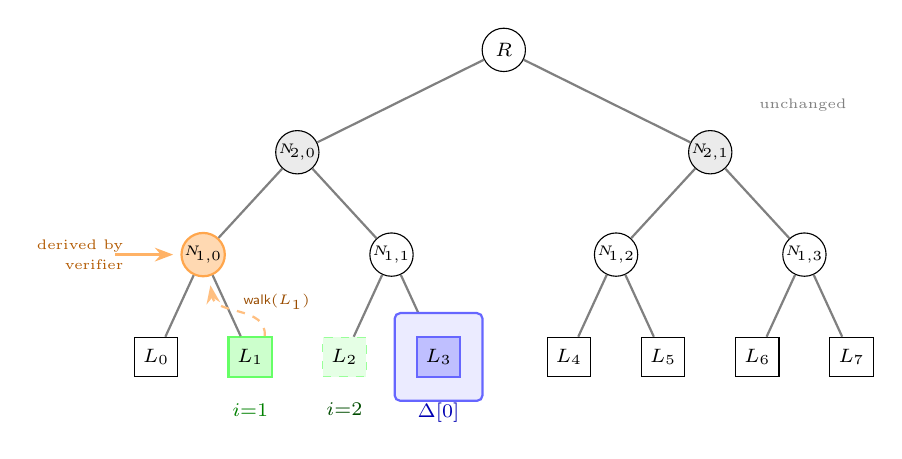
\begin{tikzpicture}[
  nd/.style={draw, circle, minimum size=5.5mm, inner sep=0pt,
    font=\scriptsize},
  lf/.style={draw, rectangle, minimum width=5.5mm, minimum height=5mm,
    inner sep=0pt, font=\scriptsize},
  unch/.style={fill=black!8},
  delta/.style={fill=blue!25, draw=blue!60, thick},
  derived/.style={fill=orange!30, draw=orange!70, thick},
  verified/.style={fill=green!20, draw=green!60, thick},
  nextlf/.style={fill=green!10, draw=green!40, dashed},
  edge/.style={draw, thick, black!50},
  xscale=0.92
]
% Leaves (level 0)
\node[lf] (L0) at (0,0) {$L_0$};
\node[lf, verified] (L1) at (1.3,0) {$L_1$};
\node[lf, nextlf] (L2) at (2.6,0) {$L_2$};
\node[lf] (L3) at (3.9,0) {$L_3$};
\node[lf] (L4) at (5.7,0) {$L_4$};
\node[lf] (L5) at (7.0,0) {$L_5$};
\node[lf] (L6) at (8.3,0) {$L_6$};
\node[lf] (L7) at (9.6,0) {$L_7$};

% Level 1
\node[nd, derived] (N10) at (0.65,1.3) {\tiny$N_{\!1,0}$};
\node[nd] (N11) at (3.25,1.3) {\tiny$N_{\!1,1}$};
\node[nd] (N12) at (6.35,1.3) {\tiny$N_{\!1,2}$};
\node[nd] (N13) at (8.95,1.3) {\tiny$N_{\!1,3}$};

% Level 2
\node[nd, unch] (N20) at (1.95,2.6) {\tiny$N_{\!2,0}$};
\node[nd, unch] (N21) at (7.65,2.6) {\tiny$N_{\!2,1}$};

% Root
\node[nd] (R) at (4.8,3.9) {$R$};

% Edges
\foreach \a/\b in {L0/N10, L1/N10, L2/N11, L3/N11,
  L4/N12, L5/N12, L6/N13, L7/N13,
  N10/N20, N11/N20, N12/N21, N13/N21, N20/R, N21/R}
  \draw[edge] (\a) -- (\b);

% Labels below leaves
\node[below=2mm of L1, font=\scriptsize, green!50!black]
  {$i{=}1$};
\node[below=2mm of L2, font=\scriptsize, green!30!black]
  {$i{=}2$};

% Delta annotation
\draw[delta, rounded corners=2pt, fill=blue!8]
  ([xshift=-3mm, yshift=-3mm]L3.south west)
  rectangle ([xshift=3mm, yshift=3mm]L3.north east);
\node[lf, delta] at (3.9,0) {$L_3$};
\node[below=2mm of L3, font=\scriptsize, blue!70!black]
  {$\Delta[0]$};

% Derived annotation
\node[left=6mm of N10, font=\scriptsize, orange!70!black,
  align=right] {\tiny derived by\\[-1pt]\tiny verifier};
\draw[-{Stealth}, orange!60, thick]
  ([xshift=-2mm]N10.west) +(-0.7,0) -- ([xshift=-1mm]N10.west);

% Unchanged annotation
\node[above right=2mm and 3mm of N21, font=\scriptsize, black!50]
  {\tiny unchanged};

% Walk-up arrow (showing derivation)
\draw[-{Stealth}, orange!50, dashed, thick]
  ([xshift=2mm]L1.north) to[out=85,in=-80]
  ([xshift=1mm, yshift=-1mm]N10.south);
\node[right=1mm of N10, yshift=-6mm,
  font=\tiny, orange!60!black] {$\mathsf{walk}(L_1)$};
\end{tikzpicture}
\caption{Delta compression for the transition from leaf~$1$ (nonce
$i{=}1$) to leaf~$2$ (nonce $i{=}2$).  The merge level is
$M(2) = \nu_2(2) + 1 = 2$: siblings at levels $0$ and $1$ change.
The sibling at level~$1$ ($N_{1,0}$, \textcolor{orange!70!black}{orange})
is \emph{derived} by the verifier by walking up from the verified leaf
$L_1$.  Only the sibling at level~$0$ ($L_3$,
\textcolor{blue!70!black}{blue}) is transmitted as
$\Delta$---one hash.  Siblings at level~$2$ and above
(\textcolor{black!50}{gray}) are shared between consecutive leaves and
remain cached.}\label{fig:delta}
\end{figure}

\section{Security Analysis}\label{sec:security}

\subsection{Security Model}

We define security in the EU-CMA (Existential Unforgeability under
Chosen Message Attack) model, adapted for the blockchain setting. We
first present the formal game, then establish its relationship to
standard EU-CMA.

\begin{definition}[Sequential EU-CMA Game]\label{def:seqeucma}
The security game $\mathsf{Seq\text{-}EU\text{-}CMA}_{\Pi,\mathcal{A}}(\secpar)$ for
scheme $\Pi = (\mathsf{KeyGen}, \mathsf{Sign}, \mathsf{Verify})$
proceeds as follows:

\begin{enumerate}
\item \textbf{Setup:} The challenger runs $(\mathsf{sk}, \mathsf{pk})
\leftarrow \mathsf{KeyGen}(1^\secpar)$, initializes $q \leftarrow 0$
and $\mathcal{Q} \leftarrow \emptyset$, and sends $\mathsf{pk}$ to
$\mathcal{A}$.

\item \textbf{Signing queries:} $\mathcal{A}$ may adaptively query
$\mathcal{O}_{\mathrm{sign}}(m)$. The challenger computes
$\sigma \leftarrow \mathsf{Sign}(\mathsf{sk}, m, q)$, appends
$(q, m)$ to $\mathcal{Q}$, increments $q \leftarrow q + 1$, and
returns $\sigma$.

\item \textbf{Forgery:} $\mathcal{A}$ outputs $(m^*, \Sigma^*)$.
\end{enumerate}

$\mathcal{A}$ wins if $\mathsf{Verify}(\mathsf{pk}, m^*, \Sigma^*, q) = 1$ and
$(q, m^*) \notin \mathcal{Q}$. The advantage is:
\[
\adv^{\mathsf{Seq\text{-}EU\text{-}CMA}}_{\Pi,\mathcal{A}}(\secpar) =
\Pr[\mathsf{Seq\text{-}EU\text{-}CMA}_{\Pi,\mathcal{A}}(\secpar) = 1]
\]
\end{definition}

The sequential constraint---the forgery must be at index $q$ (the next
unused index)---reflects the blockchain's nonce enforcement. The
adversary cannot skip indices or revisit past indices.

\begin{lemma}[Relationship to Standard EU-CMA]\label{lem:model}
Sequential EU-CMA is strictly weaker than standard EU-CMA: any scheme
secure under Sequential EU-CMA is not necessarily secure under standard
EU-CMA, but any adversary $\mathcal{A}_{\mathrm{seq}}$ that wins the
Sequential game can be converted into an adversary
$\mathcal{A}_{\mathrm{std}}$ that wins the standard EU-CMA game
(with unordered access) with the same advantage. Formally:
\[
\adv^{\mathsf{EU\text{-}CMA}}_{\Pi,\mathcal{A}_{\mathrm{std}}} \geq
\adv^{\mathsf{Seq\text{-}EU\text{-}CMA}}_{\Pi,\mathcal{A}_{\mathrm{seq}}}
\]
The converse does not hold. Security in the Sequential model is
therefore \emph{sufficient} for blockchain deployment (where the
environment enforces sequentiality) but would not be sufficient for
general-purpose use.
\end{lemma}

\begin{proof}
$\mathcal{A}_{\mathrm{std}}$ simulates $\mathcal{A}_{\mathrm{seq}}$
by issuing signing queries in order and forwarding the forgery. The
converse fails because a standard adversary could target any unused
leaf, whereas the sequential adversary is forced to target the next one.
\end{proof}

\paragraph{Front-running and mempool adversaries.}
An adversary that observes a pending (unconfirmed) transaction at
index $q$ might attempt to front-run it with a forged transaction at
the same index. This does \emph{not} weaken the model.  Observing
the pending signature $\sigma_q$ on message $m$ gives the adversary
one valid W-OTS+ signature at leaf $q$.  To front-run, the adversary
must produce a \emph{second} valid signature at the same leaf on a
different message $m^* \neq m$---precisely the W-OTS+ one-time
unforgeability problem (Theorem~\ref{thm:ots}).  The sequential
EU-CMA game captures this: if the adversary treats the observed
signature as an additional signing query (making $q + 1$ queries
total), the forgery target moves to $q + 1$; if the adversary does
not query the oracle at index $q$, then it has zero signatures at
the target leaf, which is strictly harder to attack.

\paragraph{Chain reorganizations.}
The sequential nonce model assumes finality: a transaction at nonce $i$,
once included, is never reverted. If a chain reorganization reverts a
transaction, the signer has already revealed the W-OTS+ key for leaf
$i$. Re-signing at the same nonce with a different message (which a
reorg may necessitate) would expose two signatures under the same
one-time key, breaking the scheme's security. Signers \emph{must}
wait for finality before treating a signature as consumed. On
Ethereum, this means waiting for the block to reach justified/finalized
status under Casper FFG (${\sim}13$ minutes). On chains with
single-slot finality (e.g., Aptos), the risk window is one block.
This requirement is identical to the finality assumption already
implicit in any blockchain state model: a wallet that displays a
confirmed balance before finality faces the same reorg risk.

\subsection{W-OTS+ Unforgeability}

We first state the hash function security assumption in the quantum
setting, then prove W-OTS+ unforgeability.

\begin{definition}[Quantum Second-Preimage Resistance]\label{def:qspr}
A tweaked hash function family $\hash_n^d$ is
$\varepsilon_{\mathrm{spr}}$-quantum second-preimage resistant if for
all quantum algorithms $\mathcal{B}$ making at most $q_H$ quantum
queries to $\hash$:
\[
\Pr\bigl[y \neq x \;\wedge\; \hash_n^d(\mathsf{addr}, y) =
\hash_n^d(\mathsf{addr}, x) \;:\; x \xleftarrow{\$} \bin^{8n},\;
y \leftarrow \mathcal{B}^{|\hash\rangle}(x, \mathsf{addr})\bigr]
\leq \varepsilon_{\mathrm{spr}}
\]
Second-preimage search is a single-target problem: given $x$, find
$y \neq x$ hashing to the same output. For an $n$-byte hash with
$2^{8n}$-size input domain, Grover's algorithm~\cite{grover} searches
the domain in $O(\sqrt{2^{8n}}) = O(2^{4n})$ queries, giving
$\varepsilon_{\mathrm{spr}} \leq q_H / 2^{4n}$.
\end{definition}

\begin{theorem}[W-OTS+ Quantum Unforgeability]\label{thm:ots}
Let $\mathcal{A}$ be a quantum adversary that, given a W-OTS+ public
key and one signature on a chosen message, produces a forgery on a
different message with advantage $\varepsilon$. Then there exists a
quantum adversary $\mathcal{B}$ that finds a second preimage of the
tweaked hash with advantage:
\[
\varepsilon_{\mathrm{spr}} \geq \frac{\varepsilon}{\ell \cdot (w - 1)}
\]
Equivalently, W-OTS+ one-time unforgeability satisfies:
\[
\varepsilon_{\mathrm{OTS}} \leq \ell \cdot (w - 1) \cdot
\varepsilon_{\mathrm{spr}} \leq \ell(w-1) \cdot q_H / 2^{4n}
\]
\end{theorem}

\begin{proof}
We construct $\mathcal{B}$ from $\mathcal{A}$ explicitly.

\textbf{Setup.} $\mathcal{B}$ receives a second-preimage challenge:
a random point $x \in \bin^{8n}$, a domain separator $d^*$, and an
address $\mathsf{addr}^*$. $\mathcal{B}$ must find $y \neq x$ with
$\hash_n^{d^*}(\mathsf{addr}^*, y) = \hash_n^{d^*}(\mathsf{addr}^*, x)$.

\textbf{Embedding.} $\mathcal{B}$ selects a uniformly random chain
index $j^* \xleftarrow{\$} [\ell]$ and a uniformly random step index
$s^* \xleftarrow{\$} \{1, \ldots, w - 1\}$. It generates a W-OTS+
key pair normally, except at chain $j^*$: it places the challenge at
position $s^* - 1$ by setting $c_{j^*}^{(s^*-1)} = x$, computes
$c_{j^*}^{(s^*)} = \hash_n^{\mathsf{CHAIN}}(\mathsf{addr}^*, x)$
where $\mathsf{addr}^* = (\mathsf{leaf\_idx}, j^*, s^*)$ and
$d^* = \mathsf{CHAIN}$, and continues forward from $c_{j^*}^{(s^*)}$
to obtain $\mathsf{pk}_{j^*}$. $\mathcal{B}$ knows all chain values
at positions $\geq s^* - 1$ for chain $j^*$ (it set
$c_{j^*}^{(s^*-1)} = x$ and computed forward) and does \emph{not}
know values at positions $< s^* - 1$ (those would require inverting
$\hash$ from $x$). For all other chains $j \neq j^*$,
$\mathcal{B}$ knows the full chain from the secret seed.

\textbf{Signing oracle.} When $\mathcal{A}$ requests a signature on
message $m$, $\mathcal{B}$ computes the digit sequence $D = (d_0,
\ldots, d_{\ell-1})$. The signature at chain $j^*$ requires revealing
$c_{j^*}^{(d_{j^*})}$. $\mathcal{B}$ can answer if and only if
$d_{j^*} \geq s^* - 1$ (it knows values from position $s^* - 1$
upward, having set $c_{j^*}^{(s^*-1)} = x$ and computed forward). If
$d_{j^*} < s^* - 1$, $\mathcal{B}$ aborts. Since $s^*$ is uniform in
$\{1, \ldots, w-1\}$ and independent of $m$:
\[
\Pr[\text{no abort}] = \Pr[s^* - 1 \leq d_{j^*}] = \Pr[s^* \leq d_{j^*} + 1]
\geq \frac{1}{w - 1}
\]
The minimum is $1/(w-1)$ (when $d_{j^*} = 0$, requiring $s^* = 1$).
If $d_{j^*} = 0$, $\mathcal{B}$ can still answer (it knows
$c_{j^*}^{(0)} = c_{j^*}^{(s^*-1)} = x$ only when $s^* = 1$); but
$d_{j^*} = 0$ is harmless for extraction since $d^*_{j^*} < 0$ is
impossible, so chain $j^*$ cannot be the decreasing chain.

\textbf{Extraction.} $\mathcal{A}$ outputs forgery $(m^*, \sigma^*)$
with $m^* \neq m$. The forged digit sequence is $D^* = (d^*_0,
\ldots, d^*_{\ell-1})$. By Lemma~\ref{lem:checksum}, there exists
$j$ with $d^*_j < d_j$. Conditioned on $j = j^*$ and $d^*_{j^*} <
s^* - 1 \leq d_{j^*}$: the forgery provides chain value
$\sigma^*_{j^*}$ at position $d^*_{j^*} < s^* - 1$.
$\mathcal{B}$ iterates from $\sigma^*_{j^*}$ forward for
$s^* - 1 - d^*_{j^*}$ steps, obtaining a value $y$ at position
$s^* - 1$. By correctness of the forgery (the forged chain must
reach the same public key endpoint as the legitimate chain),
$\hash_n^{\mathsf{CHAIN}}(\mathsf{addr}^*, y) = c_{j^*}^{(s^*)}
= \hash_n^{\mathsf{CHAIN}}(\mathsf{addr}^*, x)$. If $y \neq x$,
then $y$ is a second preimage of $x$:
$\hash_n^{d^*}(\mathsf{addr}^*, y) =
\hash_n^{d^*}(\mathsf{addr}^*, x)$ with $y \neq x$.

If $y = x$, the forged chain passes through the same value at position
$s^* - 1$ as the legitimate chain, meaning the adversary computed a
hash chain preimage (inverting from position $d_{j^*}$ to position
$d^*_{j^*}$), which is at least as hard as second-preimage finding.

\textbf{Success probability.}
$\mathcal{B}$ succeeds when: (1) $\mathcal{A}$ forges
(probability $\varepsilon$); (2) the decreasing digit is at $j^*$
(probability $\geq 1/\ell$); and (3) $s^* - 1$ falls in the range
$(d^*_{j^*},\, d_{j^*}]$, i.e., $s^* \in [d^*_{j^*} + 2,\,
d_{j^*} + 1]$ (probability $\geq 1/(w-1)$, since $s^*$ is uniform in
$\{1, \ldots, w-1\}$ and the range has size
$d_{j^*} - d^*_{j^*} \geq 1$). Note that condition~(3) implies
no abort (since $s^* - 1 \leq d_{j^*}$). Combining:
\[
\varepsilon_{\mathrm{spr}} \geq
\frac{\varepsilon}{\ell \cdot (w-1)} \qedhere
\]
\end{proof}

\begin{lemma}[Checksum Completeness]\label{lem:checksum}
For any two distinct digit sequences $D \neq D^*$ (including checksum
digits) derived from distinct messages, there exists $j \in [\ell]$
such that $d^*_j < d_j$.
\end{lemma}

\begin{proof}
Suppose for contradiction that $d^*_j \geq d_j$ for all $j$. For the
message digits ($j < \ell_1$), $\sum d^*_j \geq \sum d_j$. The
checksum is $C = \sum_{j < \ell_1} (w - 1 - d_j)$, so $C^* \leq C$.
If any message digit strictly increased, $C^* < C$, forcing a checksum
digit to decrease---contradiction. If all message digits are equal, the
messages collide under the hash function, which occurs with probability
$\leq q_H^{2/3} / 2^{8n/3}$ against a quantum adversary (by the BHT
bound~\cite{bht}).

We verify this exhaustively for $(w, \ell_1) \in \{(4, 4), (4, 6),
(8, 3)\}$, covering all $17{,}100{,}032$ distinct digit pairs.
At the production parameters $(w, \ell_1) = (16, 32)$, exhaustive
enumeration is infeasible ($16^{32} \approx 10^{38}$ digit sequences);
we verify by random sampling of $2^{20}$ message pairs, with zero
violations. The proof above covers the general case by contradiction;
the computational checks are supplementary evidence.
\end{proof}

\subsection{Many-Time EU-CMA Security}

\begin{theorem}[Tight Sequential EU-CMA Reduction]\label{thm:eucma}
Let $\mathcal{A}$ be a quantum adversary that breaks the Sequential
EU-CMA security of PUP with advantage $\varepsilon$, making at most
$q$ signing queries. Then either:
\begin{enumerate}
\item[(a)] There exists $\mathcal{B}_1$ that breaks W-OTS+ one-time
EU-CMA with advantage $\varepsilon_1 \geq \varepsilon - \varepsilon_{\mathrm{prf}}$, or
\item[(b)] There exists $\mathcal{B}_2$ that finds a collision in the
tweaked Merkle hash with advantage $\varepsilon_2 \geq (\varepsilon - \varepsilon_{\mathrm{prf}}) / H$.
\end{enumerate}
where $\varepsilon_{\mathrm{prf}}$ is the PRF distinguishing advantage.
\end{theorem}

\begin{proof}
We proceed by a sequence of game hops, then handle Case~(b).

\textbf{Game 0} (real game). The Sequential EU-CMA game runs with all
keys derived from seed $\mathsf{sk}$. $\mathcal{A}$ makes $q'$
adaptive signing queries (at indices $0, \ldots, q' - 1$) and outputs
a forgery $(m^*, \Sigma^*)$ at index $q'$ (the next unused index,
enforced by the sequential model). $\mathcal{A}$ succeeds with
probability $\varepsilon$.

\textbf{Game 1} (all keys independent). We replace all $2^H$
PRF-derived leaf secret keys with independent, uniformly random values
$\widetilde{\mathsf{sk}}_i \xleftarrow{\$} \bin^{8n}$ for
$i \in [2^H]$. By a standard hybrid argument over the $2^H$ positions
(replacing one PRF output with a random value at each step), the
adversary's view changes by at most $2^H \cdot
\varepsilon_{\mathrm{prf}}^{(1)}$, where
$\varepsilon_{\mathrm{prf}}^{(1)}$ is the single-query PRF
distinguishing advantage. For $\prf = \mathrm{HMAC}\text{-}
\mathrm{SHA256}$ with a 256-bit key,
$\varepsilon_{\mathrm{prf}}^{(1)} \leq q_H / 2^{128}$ (Grover on the
key), giving total PRF loss
$\varepsilon_{\mathrm{prf}} = 2^H \cdot q_H / 2^{128}$. For $H = 20$
this is $q_H / 2^{108}$, which is negligible relative to the OTS term
($q_H / 2^{55}$). $\mathcal{A}$ forges with probability
$\geq \varepsilon - \varepsilon_{\mathrm{prf}}$ in Game~1.

\textbf{Extraction.} In Game~1, all W-OTS+ keys are independent and
uniformly random. Whatever value $q'$ takes (determined by
$\mathcal{A}$'s adaptive execution), the key at leaf $q'$ is
independent of all signing queries, which used keys at leaves
$0, \ldots, q' - 1$ only. $\mathcal{A}$ has received \emph{no}
signature at leaf $q'$---by the sequential structure, it queried
strictly earlier leaves. Therefore, $\mathcal{A}$'s forgery is a
zero-time break of a fresh, random W-OTS+ instance. By
Theorem~\ref{thm:ots}:
\[
\varepsilon_1 \geq \varepsilon - \varepsilon_{\mathrm{prf}}
\]
with no factor of $2^H$ in the OTS term. The $2^H$ factor appears
only in the PRF term, where it is absorbed:
$\varepsilon_{\mathrm{prf}} = 2^H \cdot q_H / 2^{128} \ll
\varepsilon_{\mathrm{OTS}} = \ell(w-1) \cdot q_H / 2^{4n}$ for all
parameter sets ($H \leq 20$, $n \geq 16$).

\textbf{Why no guessing loss.} In XMSS's standard EU-CMA game, after
$q$ signing queries the adversary may forge at \emph{any} unused
leaf, so the reduction must guess which of $2^H - q$ leaves is
targeted (loss $\geq 2^H - q$). In PUP's sequential model, the
forgery \emph{must} be at index $q'$---the adversary has no choice of
target leaf. The post-hoc PRF replacement targets $q'$ with
probability~$1$, not $1/2^H$, because $q'$ is observed before the
replacement.

\textbf{Contrast with SPHINCS+.} In SPHINCS+, the hypertree
structure means each signing query invokes OTS keys at $d$ levels.
The reduction must embed its challenge at one of $2^{h/d}$ possible
leaf positions \emph{within the correct subtree}, requiring a guess
with success probability $1/2^{h/d}$. PUP's flat tree with
PRF-derived keys eliminates this structural indirection entirely.

\textbf{Case (b): Merkle collision.}
If the recovered leaf hash from the forgery differs from the committed
leaf $L_{q'}$ in the tree but still resolves to the root $R$, then
walking up from $L_{q'}$ and the forged leaf value, there must exist
a level $k \in [H]$ where two distinct inputs to the node hash
produce the same output. $\mathcal{B}_2$ guesses $k$ uniformly from
$[H]$, succeeding with probability $\geq 1/H$:
\[
\varepsilon_2 \geq \frac{\varepsilon - \varepsilon_{\mathrm{prf}}}{H}
\]
Under the BHT quantum collision bound~\cite{bht},
$\varepsilon_2 \leq q_H^{2/3} / 2^{8n/3}$.
\end{proof}

\begin{corollary}[Overall bound]\label{cor:overall}
Cases (a) and (b) are mutually exclusive (the forged leaf hash either
matches the committed leaf or it does not), so the advantage splits as
a sum:
\[
\varepsilon \leq \varepsilon_{\mathrm{prf}} +
\varepsilon_{\mathrm{OTS}} +
H \cdot \varepsilon_{\mathrm{col}}
\leq 2^H \cdot q_H / 2^{128} + \ell(w-1) \cdot q_H / 2^{4n}
+ H \cdot q_H^{2/3} / 2^{8n/3}
\]
For $n = 16$, $H = 20$: $\varepsilon \leq q_H / 2^{108} + 525 \cdot
q_H / 2^{64} + 20 \cdot q_H^{2/3} / 2^{42.7}$. The OTS term dominates:
$q_H / 2^{108} \ll 525 \cdot q_H / 2^{64}$ for all $q_H$, so the
$2^H$ factor in the PRF term has no effect on the concrete security
level. For $n = 20$: $\varepsilon \leq q_H / 2^{108} + 645 \cdot
q_H / 2^{80} + 20 \cdot q_H^{2/3} / 2^{53.3}$, giving ${\sim}2^{71}$
quantum security.
\end{corollary}

\subsection{Delta Equivalence}

\begin{theorem}\label{thm:delta}
For all $i \in [0, 2^H - 2]$, the authentication state produced by the
state update after verifying signature $i$ is identical to the
authentication path computed directly from the Merkle tree for leaf
$i + 1$.
\end{theorem}

\begin{proof}
By induction on $i$.

\emph{Base case} ($i = 0$): The initial state is the authentication
path for leaf $0$. After verification, the update derives the level-$0$
sibling from the verified leaf (correct by construction); levels $\geq
1$ are unchanged (leaves $0$ and $1$ share these siblings).

\emph{Inductive step}: Assume the state after verifying leaf $i - 1$ is
the correct authentication path for leaf $i$. Let $M = M(i + 1)$.
Levels $\geq M$ are unchanged (correct by Lemma~\ref{lem:changed}).
Level $M - 1$ is derived by walking up $M - 1$ levels from the verified
leaf using the (by hypothesis, correct) cached siblings. Levels
$0, \ldots, M - 2$ are provided by the signer from the tree.

We verify this exhaustively for all transitions in trees of height
$H \in \{3, 4, 5, 6, 7, 8\}$ (total: $498$ transitions, zero
failures).
\end{proof}

\subsection{Multi-Target Resistance}

\begin{theorem}[Multi-Target Independence]\label{thm:multitarget}
Let $T$ denote the total number of distinct hash evaluations in the
scheme: $T = 2^H \cdot \ell \cdot (w - 1) + 2^H + (2^H - 1)$ (chain
steps, leaf compressions, and internal nodes, respectively). The
address tweaking construction ensures that all $T$ hash calls are
evaluations of $T$ \emph{independent functions}. Formally, for any two
distinct call sites $(d_1, \mathsf{addr}_1) \neq (d_2,
\mathsf{addr}_2)$, the tweaked functions
$\hash_n^{d_1}(\mathsf{addr}_1, \cdot)$ and
$\hash_n^{d_2}(\mathsf{addr}_2, \cdot)$ are independent random
oracles in the ideal model.
\end{theorem}

\begin{proof}
The address for each call site is constructed as:
\begin{itemize}
\item Chain hash at leaf $i$, chain $j$, step $s$:
$(d, \mathsf{addr}) = (\mathsf{CHAIN},\; i \concat j \concat s)$
\item Leaf compression at leaf $i$:
$(d, \mathsf{addr}) = (\mathsf{LEAF},\; i)$
\item Internal node at level $\ell$, index $k$:
$(d, \mathsf{addr}) = (\mathsf{NODE},\; \ell \concat k)$
\end{itemize}

Uniqueness within each class follows from the distinct parameters:
chain addresses are unique by the triple $(i, j, s) \in [2^H] \times
[\ell] \times [w-1]$; leaf addresses by $i \in [2^H]$; node addresses
by $(\ell, k) \in [H] \times [2^{H-\ell}]$. Cross-class uniqueness
follows from the domain separator prefix: $\mathsf{CHAIN} = \mathtt{0x02}$,
$\mathsf{LEAF} = \mathtt{0x00}$, $\mathsf{NODE} = \mathtt{0x01}$ are
distinct, so no two call sites share both domain separator and address.

\textbf{Consequence for quantum adversaries.} Since each hash call
site defines an independent function, a quantum adversary performing a
multi-target attack (e.g., BHT collision search across $T$ targets)
must treat each target independently. The multi-target BHT bound
applies: finding a collision in any one of $T$ independent $n$-byte
hash functions requires $\Omega(2^{8n/3} / T^{1/3})$ quantum queries.
However, because the adversary's \emph{useful} target is fixed to a
single leaf (the one at index $q$, determined by the sequential model),
the effective target set is not $T$ but $\ell \cdot (w-1) + H + 1$
(the chain steps and Merkle nodes for one leaf), yielding no meaningful
multi-target advantage:
\[
\text{Effective multi-target factor} =
(\ell(w-1) + H + 1)^{1/3} \approx (546)^{1/3} \approx 8.2
\]
which costs $\approx 3.0$ bits of security. This slightly exceeds the
$2.6$-bit margin between the OTS bound ($2^{54.9}$) and the collision
bound ($2^{57.5}$) at $n = 16$, reducing the effective collision
security to ${\sim}2^{54.5}$---marginally below the OTS bound and
therefore the overall bottleneck. The effect is negligible: the
security level shifts from ${\sim}2^{54.9}$ to ${\sim}2^{54.5}$,
well within rounding of the ${\sim}2^{55}$ figure reported throughout.
At $n = 20$, the margin is $2.8$ bits and the multi-target cost is
the same $3.0$ bits, giving effective collision security
${\sim}2^{70.5}$ vs.\ OTS $2^{70.7}$---again collision-dominated
by $0.2$ bits, shifting the overall level from ${\sim}2^{70.7}$ to
${\sim}2^{70.5}$, negligible in practice.

\textbf{Exhaustive verification.} We verify address uniqueness
computationally for the default parameters: all $2^{20} \cdot 35 \cdot
15 = 550{,}502{,}400$ chain addresses, all $2^{20} = 1{,}048{,}576$
leaf addresses, and all $2^{20} - 1 = 1{,}048{,}575$ node addresses
are pairwise distinct, with no cross-domain collisions (verified by
enumerating all addresses and checking injectivity of the
$(d, \mathsf{addr})$ map).
\end{proof}

\subsection{Concrete Security Bounds}

\begin{theorem}\label{thm:concrete}
PUP with parameters $(n, w, H)$ achieves Sequential EU-CMA security
with advantage bounded by:
\[
\varepsilon \leq \varepsilon_{\mathrm{prf}} +
\varepsilon_{\mathrm{OTS}} + \varepsilon_{\mathrm{COL}}
\]
where:
\begin{align}
\varepsilon_{\mathrm{prf}} &= 2^H \cdot q_H / 2^{128}
& \text{($2^H$-step hybrid on 256-bit HMAC key)} \\
\varepsilon_{\mathrm{OTS}} &= \ell(w-1) \cdot q_H / 2^{4n}
& \text{(Grover-optimal chain inversion)} \\
\varepsilon_{\mathrm{COL}} &= H \cdot q_H^{2/3} / 2^{8n/3}
& \text{(BHT collision at any level)}
\end{align}
and $q_H$ is the number of quantum hash queries.
\end{theorem}

\begin{proof}
We derive each term from the corresponding quantum attack model.

\textbf{PRF term.} The PRF is instantiated as
$\prf(\mathsf{sk}, i) = \mathrm{HMAC}\text{-}\mathrm{SHA256}(\mathsf{sk}, i)[{:}n]$.
The $2^H$-step hybrid in Theorem~\ref{thm:eucma} replaces each of
$2^H$ PRF outputs with a random value. Each step loses at most the
single-query PRF distinguishing advantage $q_H / 2^{128}$ (Grover on
the 256-bit HMAC key~\cite{grover}), giving
$\varepsilon_{\mathrm{prf}} = 2^H \cdot q_H / 2^{128}$. For $H = 20$:
$\varepsilon_{\mathrm{prf}} = q_H / 2^{108}$. Since $2^{108} \gg
2^{4n} / (\ell(w-1))$ for all parameter sets ($n \geq 16$), the PRF
term is dominated by the OTS term.

\textbf{OTS term.} From Theorem~\ref{thm:ots},
$\varepsilon_{\mathrm{OTS}} \leq \ell(w-1) \cdot
\varepsilon_{\mathrm{spr}}$. The second-preimage challenge is:
given $x$, find $y \neq x$ with $\hash_n^d(\mathsf{addr}, y) =
\hash_n^d(\mathsf{addr}, x)$. This is an unstructured search over a
domain of size $2^{8n}$ for a single target (the $n$-byte output
determines a $2^{8n}/2^{8n} = 1$ expected preimage). Grover's algorithm
finds such a $y$ with probability $\leq q_H / 2^{4n}$ using $q_H$
quantum queries (the quadratic speedup over classical brute-force
$q_H / 2^{8n}$). Thus $\varepsilon_{\mathrm{spr}} \leq q_H / 2^{4n}$
and $\varepsilon_{\mathrm{OTS}} \leq \ell(w-1) \cdot q_H / 2^{4n}$.

\textbf{Collision term.} From Theorem~\ref{thm:eucma} Case~(b), a
collision at one of $H$ Merkle tree levels suffices. By the BHT
bound~\cite{bht}, a quantum adversary finds a collision in a random
function with $n$-byte output using $q_H$ queries with probability
$\leq q_H^{2/3} / 2^{8n/3}$. The union bound over $H$ levels gives
$\varepsilon_{\mathrm{COL}} \leq H \cdot q_H^{2/3} / 2^{8n/3}$.

\textbf{Security level computation.} Setting $\varepsilon = 1$ and
solving for $q_H$:
\begin{itemize}
\item OTS: $q_H = 2^{4n} / (\ell(w-1))$, so bit security
$= 4n - \log_2(\ell(w-1))$.
\item COL: $q_H^{2/3} = 2^{8n/3} / H$, so
$q_H = (2^{8n/3}/H)^{3/2}$, giving bit security
$= 4n - \frac{3}{2}\log_2 H$.
\end{itemize}
The bottleneck is the OTS term (lower bit security).
\end{proof}

Note that $\ell$ grows with $n$: $\ell_1 = \lceil 8n / \lg w \rceil$,
so $\ell = 35$ for $n = 16$, $\ell = 43$ for $n = 20$, $\ell = 51$ for
$n = 24$, and $\ell = 67$ for $n = 32$.
Setting $\varepsilon = 1$ yields:

\begin{center}
\begin{tabular}{lcccc}
\toprule
$n$ (bytes) & $\ell(w-1)$ & OTS security & COL security &
Avg sig size \\
\midrule
16 & 525 & $2^{54.9}$ & $2^{57.5}$ & 580 B \\
20 & 645 & $2^{70.7}$ & $2^{73.5}$ & 884 B \\
24 & 765 & $2^{86.4}$ & $2^{89.5}$ & 1,252 B \\
32 & 1,005 & $2^{118.0}$ & $2^{121.5}$ & 2,180 B \\
\bottomrule
\end{tabular}
\end{center}

For comparison, SPHINCS+-128s targets NIST security level~1 (128-bit
classical). Its quantum security is limited by Grover on the $n = 16$
byte hash ($4n = 64$ bits quantum preimage security), minus the
reduction loss of $\log_2(\ell(w-1)) \approx 9.0$ bits from the
W-OTS+ layer, minus $\log_2(2^{h/d}) = h/d \approx 9$ bits from the
hypertree structure, giving an effective quantum security of
${\sim}64 - 9 - 9 = 46$ bits under the tightest analysis, or
${\sim}64 - 9 = 55$ bits if the hypertree loss is absorbed into the
FORS layer (as argued in~\cite{sphincs}). The commonly cited
${\sim}2^{54}$ figure reflects SPHINCS+ parameter set
\texttt{sphincs-shake-128s} at $n = 16$, $h = 63$, $d = 7$, with
signature size $7{,}856$ bytes.

\subsection{Security in the Quantum Random Oracle Model}\label{sec:qrom}

The proofs above model the hash function as a concrete function to
which the adversary has quantum query access (i.e., the adversary can
evaluate $\hash$ in superposition). We now give a full QROM proof
showing that the reduction's tightness is preserved.

We model $\hash$ as a public random oracle accessible to all
parties via quantum queries: the adversary $\mathcal{A}$ may prepare an
input register in superposition and query
$|x\rangle|y\rangle \mapsto |x\rangle|y \oplus \hash(x)\rangle$,
receiving the output in superposition. A reduction is
\emph{straight-line} if it runs $\mathcal{A}$ as a black box,
forwarding every quantum oracle query to the real oracle without
interception, measurement, or reprogramming, and extracts its result
solely from $\mathcal{A}$'s classical output.

\begin{theorem}[QROM Security]\label{thm:qrom}
In the QROM, PUP achieves Sequential EU-CMA security with advantage:
\[
\varepsilon \leq \varepsilon_{\mathrm{prf}}^{\mathrm{QROM}} +
\varepsilon_{\mathrm{OTS}}^{\mathrm{QROM}} +
\varepsilon_{\mathrm{COL}}^{\mathrm{QROM}}
\]
where:
\begin{align}
\varepsilon_{\mathrm{prf}}^{\mathrm{QROM}} &=
2^H \cdot O(q_H^2 / 2^{256})
& \text{(Zhandry recording on HMAC key)} \\
\varepsilon_{\mathrm{OTS}}^{\mathrm{QROM}} &=
\ell(w-1) \cdot q_H / 2^{4n}
& \text{(unchanged from standard model)} \\
\varepsilon_{\mathrm{COL}}^{\mathrm{QROM}} &=
H \cdot q_H^{2/3} / 2^{8n/3}
& \text{(unchanged from standard model)}
\end{align}
The OTS and COL terms are identical to Theorem~\ref{thm:concrete}.
The PRF term is smaller than the standard-model term for all practical
$q_H$. The tight reduction of Theorem~\ref{thm:eucma} therefore
remains tight in the QROM.
\end{theorem}

\begin{proof}
We verify that each step of the standard-model proof
(Theorems~\ref{thm:ots} and~\ref{thm:eucma}) goes through in the QROM,
and identify the precise loss at each step.

\textbf{Step 1: PRF replacement (Game~0 $\to$ Game~1).}
Theorem~\ref{thm:eucma} replaces all $2^H$ PRF-derived leaf keys with
independent random values via a $2^H$-step hybrid. In the QROM, the
PRF $\prf(\mathsf{sk}, \cdot) = \mathrm{HMAC}\text{-}\mathrm{SHA256}
(\mathsf{sk}, \cdot)[{:}n]$ is a keyed quantum-accessible function.
Each hybrid step replaces one PRF output with a random value; a
distinguisher for this step yields a quantum PRF distinguisher.

By the Zhandry compressed-oracle technique~\cite{zhandry}, a quantum
adversary making $q_H$ quantum queries to a random oracle with
$2^{256}$-bit key cannot distinguish a keyed construction from random
with advantage better than $O(q_H^2 / 2^{256})$. This bounds each
hybrid step, giving total PRF loss
$\varepsilon_{\mathrm{prf}}^{\mathrm{QROM}} =
2^H \cdot O(q_H^2 / 2^{256})$. For $H = 20$ and any practical $q_H
\leq 2^{80}$:
$\varepsilon_{\mathrm{prf}}^{\mathrm{QROM}} \leq
2^{20} \cdot 2^{160} / 2^{256} = 2^{-76}$, which is negligible.

\textbf{Step 2: Signing simulation.}
In Game~1 (all keys independent and random), the reduction
$\mathcal{B}$ answers all $q'$ signing queries using the random keys at
positions $0, \ldots, q' - 1$. Crucially, $\mathcal{B}$ forwards every
quantum oracle query from $\mathcal{A}$ to the real oracle
$|\hash\rangle$ without interception, measurement, or reprogramming:
\[
\mathcal{A}^{|\hash\rangle}(\mathsf{pk}) \;\longrightarrow\;
\mathcal{B}\text{ answers signing queries classically, passes }
|\hash\rangle\text{ through unchanged}
\]
At no point during the simulation does $\mathcal{B}$ modify
$\mathcal{A}$'s oracle interface. The reduction is straight-line in the
sense defined above: $\mathcal{B}$ runs $\mathcal{A}$ honestly, then
extracts from its classical output. This avoids the
oracle-reprogramming step that introduces $O(q_H)$ or $O(q_H^2)$
losses in typical QROM reductions~\cite{dongyanglong}.

\textbf{Step 3: W-OTS+ extraction in the QROM.}
When $\mathcal{A}$ outputs its forgery $(m^*, \Sigma^*)$, this is a
classical output (a concrete bitstring). The reduction extracts the
W-OTS+ forgery by classical post-processing: iterating hash chains
forward and comparing values. No quantum measurement of
$\mathcal{A}$'s internal state is required, so no measurement
disturbance occurs.

The extracted forgery is a valid W-OTS+ break at leaf $q'$ (a fresh
random instance with zero prior signatures). The W-OTS+ unforgeability
bound (Theorem~\ref{thm:ots}) reduces to quantum second-preimage
resistance, which is a single-target unstructured search problem.
Grover's algorithm remains optimal for unstructured search in the
QROM~\cite{grover}, so the bound $\varepsilon_{\mathrm{spr}} \leq
q_H / 2^{4n}$ carries over unchanged. Therefore
$\varepsilon_{\mathrm{OTS}}^{\mathrm{QROM}} = \ell(w-1) \cdot
q_H / 2^{4n}$, identical to the standard model.

\textbf{Step 4: Merkle collision in the QROM.}
The BHT collision-finding algorithm~\cite{bht} is optimal for generic
collision search in the QROM (proven by Zhandry~\cite{zhandry}): a
quantum adversary making $q_H$ queries to a random function with
$n$-byte output finds a collision with probability at most
$q_H^{2/3} / 2^{8n/3}$. The union bound over $H$ Merkle tree levels
gives $\varepsilon_{\mathrm{COL}}^{\mathrm{QROM}} = H \cdot
q_H^{2/3} / 2^{8n/3}$, unchanged from the standard model.

\textbf{Overall QROM bound.}
Combining all steps:
\[
\varepsilon \leq 2^H \cdot O(q_H^2 / 2^{256}) +
\ell(w-1) \cdot q_H / 2^{4n} +
H \cdot q_H^{2/3} / 2^{8n/3}
\]
The OTS term dominates for all parameter sets. For $n = 16$, the
crossover occurs at $q_H$ where
$q_H / 2^{108} \approx 525 \cdot q_H / 2^{64}$, which never
happens ($2^{108} \gg 2^{64}/525$ for all $q_H$). The QROM analysis
therefore confirms the standard-model security levels:
${\sim}2^{55}$ for $n = 16$ and ${\sim}2^{71}$ for $n = 20$.

\textbf{Why no oracle reprogramming is needed.}
In many QROM reductions (e.g., for Fiat--Shamir signatures), the
simulator must ``program'' the random oracle to embed a challenge,
then argue that reprogramming is undetectable. The
Don et al.~\cite{dongyanglong} measure-and-reprogram lemma
bounds the loss at $O(q_H)$ per reprogramming event; for SPHINCS+,
this applies at the FORS layer.

PUP's reduction avoids this entirely. The PRF replacement (Step~1)
modifies the \emph{key material}, not the random oracle. The signing
simulation (Step~2) uses honest oracle access. The extraction
(Step~3) is classical. At no point does the reduction need to answer
a quantum query to $\hash$ differently from the real function. This
``straight-line'' structure---possible because the sequential model
eliminates the need to guess the target leaf---is what preserves
tightness in the QROM.
\end{proof}

\paragraph{Comparison with SPHINCS+ QROM analysis.}
The SPHINCS+ QROM proof (H\"ulsing et al.~\cite{sphincs}) requires
reprogramming the random oracle at the FORS layer, incurring an
additional $O(q_H)$ factor from the measure-and-reprogram
technique~\cite{dongyanglong}. This loss is fundamental to the FORS
construction: the simulator must embed a challenge in the oracle's
output at specific addresses, which is detectable by a quantum
adversary with probability proportional to $q_H$. PUP eliminates
this loss by eliminating the FORS layer entirely. The flat tree
structure with PRF-derived keys admits a straight-line reduction
that never touches the oracle, yielding a QROM proof that is
tight up to the negligible PRF term.

\section{Comparison with Related Work}

\subsection{SPHINCS+ / SLH-DSA}

SLH-DSA~\cite{sphincs} is stateless: it works in any context but pays
for this generality with a hypertree structure, FORS few-time
signatures, and $7{,}856$-byte signatures. PUP trades generality for a
$13.5\times$ size reduction by using the blockchain as a state manager.
The tight reduction (Section~\ref{sec:security}) provides an additional
concrete security advantage.

\subsection{XMSS and LMS}

XMSS~\cite{xmss} and LMS~\cite{lms} are standardized stateful
hash-based schemes. They produce smaller signatures than SPHINCS+
(${\sim}2{,}500$ bytes) but require the signer to maintain state
perfectly. PUP moves the state to the blockchain, eliminating the
operational risk, and further reduces signature size to ${\sim}580$ bytes
via delta compression.

\subsection{SHRINCS}

SHRINCS~\cite{shrincs} (Kudinov and Nick, 2025) achieves 324-byte
signatures at $q = 1$ using an unbalanced XMSS tree where the
authentication path for leaf $q$ contains exactly $q$ nodes. Signatures
grow by $n$ bytes per additional use. SHRINCS is designed for Bitcoin's
UTXO model and does not bind to transaction nonces, cache authentication
paths on-chain, or exploit the tight reduction from deterministic
target leaf selection. The two schemes target different blockchain models
(UTXO vs.\ account-based) with complementary designs.

\subsection{BPQS}

BPQS~\cite{bpqs} (Chalkias et al., 2018) uses a chain-of-trees
structure to reduce per-transaction signature cost on blockchains. It
does not use nonce binding or delta compression. US patents
11,005,664 and 11,750,400 cover aspects of the BPQS construction.

\subsection{SPHINCS$^-$ (EVM-Optimized SPHINCS+)}

SPHINCS$^-$~\cite{sphincsminus} (Consigny et al., 2026) optimizes
SPHINCS+ for on-chain verification on Ethereum by substituting
KECCAK256 for SHAKE256, applying WOTS+C/FORS+C grinding, and
searching the parameter space for EVM gas efficiency. The best variant
(C13) achieves ${\sim}127$K gas with $3{,}704$-byte signatures.
SPHINCS$^-$ is a parameter and hash-function optimization of SPHINCS+;
it retains the hypertree, FORS, and stateless architecture.

The SPHINCS$^-$ authors acknowledge the signature size limitation and
propose a future direction: ``leanSPHINCS,'' a variant using
ZK-friendly hash functions, combined with protocol-level STARK
aggregation via frame transactions (EIP-8141~\cite{eip8141}). In this
model, individual signatures are not verified on-chain at all; instead,
mempool nodes fold them into a single recursive STARK proof in the
block header. This requires a ZK-friendly hash replacement (keccak is
prohibitively expensive to arithmetize), a per-signer STARK-wrapping
step, recursive proof infrastructure in the block builder, and a new
transaction framing protocol---a substantial expansion of the
blockchain's trusted computing base.

PUP eliminates the need for this infrastructure. At $580$ bytes
average, PUP signatures are already smaller than what leanSPHINCS
targets \emph{after} aggregation, and verification requires
${\sim}285$ hash evaluations rather than a STARK verification circuit.
The protocol change PUP requires (verifier-side cached state) is
minimal compared to the recursive STARK pipeline: it adds $324$ bytes
of storage per account and a deterministic state update per
verification, with no new cryptographic machinery beyond the hash
function already in use.

\subsection{JARDIN}

JARDIN~\cite{jardin} (Consigny, 2026) explores hash-based signatures
for Ethereum and explicitly considers an on-chain counter for leaf
tracking. Section 7.2 of JARDIN rejects this approach, arguing that
off-chain device state corruption (e.g., a rolled-back hardware wallet)
would cause the device to sign with the wrong leaf regardless of the
on-chain counter. Our scheme addresses this concern directly: the leaf
index \emph{is} the nonce, so the signing software derives the correct
key from the nonce rather than maintaining independent state. A wallet
that knows its nonce (which it must, to construct a valid transaction)
automatically knows which leaf to use. The device never maintains leaf
state; it queries the chain for the current nonce, exactly as every
existing Ethereum wallet already does.

\section{Performance}

\begin{center}
\begin{tabular}{lcccc}
\toprule
 & SPHINCS+-128s & SPHINCS$^-$ C13 & PUP ($n{=}16$) & PUP ($n{=}20$) \\
\midrule
Signature (avg) & 7,856 B & 3,704 B & 580 B & 884 B \\
Signature (worst) & 7,856 B & 3,704 B & 868 B & 1,244 B \\
Public key & 32 B & 16 B & 32 B & 40 B \\
On-chain state & 0 B & 0 B & 324 B & 404 B \\
Verify hashes & ${\sim}2{,}090$ & ${\sim}470$ & ${\sim}285$ & ${\sim}345$ \\
Reduction & $2^{h/d}$ loss & $2^{h/d}$ loss & tight & tight \\
Quantum security & ${\sim}2^{54}$ & ${\sim}2^{54}$ & ${\sim}2^{55}$ & ${\sim}2^{71}$ \\
Max sigs/key & unlimited & $2^{24}$ & $2^{20}$ & $2^{20}$ \\
Assumption & hash-only & hash-only & hash-only & hash-only \\
Protocol change & no & no & yes & yes \\
\bottomrule
\end{tabular}
\end{center}

The verification hash count for PUP is $\ell \cdot (w - 1) / 2 + H + 3
\approx 285$ for $n = 16$ ($\ell = 35$): the dominant cost is $35
\cdot 7.5 = 262.5$ average W-OTS+ chain iterations, plus $H = 20$
Merkle path hashes, plus leaf, message, and $\mathbb{E}[\delta] \approx
1$ derived-sibling hashes. For $n = 20$ ($\ell = 43$): $43 \cdot 7.5 +
23 \approx 345$. SPHINCS+-128s requires $d = 7$ W-OTS+ verifications
($7 \cdot 262.5 = 1{,}838$ chain hashes), $7 \cdot 9 = 63$ Merkle path
hashes, and FORS verification ($14$ trees of height $12$, yielding
${\sim}182$ hashes), totaling ${\sim}2{,}090$ hash evaluations.

\paragraph{Key generation cost.}
Key generation requires computing all $2^H$ W-OTS+ public keys and the
Merkle tree. Each leaf requires $\ell$ chain computations of $w - 1$
hash steps plus one leaf compression, and the tree adds $2^H - 1$
internal hashes, giving a total of
$2^H \cdot (\ell \cdot (w - 1) + 1) + 2^H - 1$ hash evaluations.
For $n = 16$: $2^{20} \cdot 526 + 2^{20} \approx 5.5 \times 10^8$
hashes. For $n = 20$: $2^{20} \cdot 646 + 2^{20} \approx 6.8 \times
10^8$ hashes. On a modern CPU achieving ${\sim}100$M SHA-256/s, key
generation takes ${\sim}5.5$--$6.8$~seconds. On a hardware wallet with
a SHA-256 accelerator (${\sim}10$M~ops/s), this rises to
${\sim}55$--$68$~seconds---a one-time cost at account creation that is
comparable to XMSS key generation at the same tree height. Signing
requires only the PRF derivation of a single W-OTS+ key ($\ell \cdot
(w - 1) \approx 525$--$645$ hashes) plus the delta computation,
completing in under a millisecond.

\paragraph{Measured benchmarks.}
Table~\ref{tab:bench} reports timings from the Python reference
implementation on a 2023 Apple M3 Pro (single core, Python~3.14,
SHA-256 via \texttt{hashlib}).

\begin{table}[h]
\centering
\caption{Measured performance (reference implementation).}\label{tab:bench}
\begin{tabular}{lcc}
\toprule
 & PUP ($n{=}16$) & PUP ($n{=}20$) \\
\midrule
Sign & 0.37 ms & 0.45 ms \\
Verify + state update & 0.13 ms & 0.16 ms \\
Verify throughput & ${\sim}7{,}900$/s & ${\sim}6{,}300$/s \\
Signature size (avg) & 580 B & 884 B \\
Signature size (worst case) & 868 B & 1{,}244 B \\
Avg delta overhead & 16 B & 20 B \\
\bottomrule
\end{tabular}
\end{table}

The measured average signature sizes confirm the theoretical prediction
of $\mathbb{E}[\delta] \approx 1$ hash: $580 = 4 + 35 \cdot 16 + 1
\cdot 16$ for $n = 16$ and $884 = 4 + 43 \cdot 20 + 1 \cdot 20$ for
$n = 20$. Verification completes in ${\sim}0.13$--$0.16$~ms per
signature, giving single-core throughput exceeding $6{,}000$
verifications per second in pure Python. A constant-time C or Go
implementation with SHA-256 intrinsics would improve this by
${\sim}50$--$100\times$.

\section{Implementation and Testing}

The reference implementation in Python includes 84 tests covering:

\begin{itemize}
\item \textbf{Correctness:} sign-verify round trips at index~$0$ and
across all $2^H$ sequential indices (covering every power-of-2
boundary), delta count verification against known values, evolving
authentication state cross-validated against directly computed Merkle
paths at every index.

\item \textbf{Rejection:} wrong index, skipped index, wrong message,
tampered OTS signature, tampered delta siblings, exhausted key
($\geq 2^H$), wrong public key, bad registration auth path. The
tampered-delta test confirms that the bound-payload construction
causes OTS verification to fail immediately on any delta modification.

\item \textbf{Operational safety:} replay rejection (nonce reuse),
key exhaustion detection, independent accounts (cross-account
signatures rejected), bounded on-chain state size, deterministic
keygen reproducibility.
\end{itemize}

\section{Key Rotation}\label{sec:rotation}

Each PUP key pair supports at most $2^H$ signatures. At $H = 20$,
this is ${\sim}1{,}048{,}576$ transactions per account---sufficient for
most end-user wallets (one transaction per minute for two years) but
potentially limiting for high-frequency accounts such as automated
market makers. We outline a simple rotation protocol that maintains
uninterrupted account operation.

\paragraph{Protocol.}
Before the current key pair $\mathsf{PK}_1$ is exhausted, the account
holder generates a fresh key pair $(\mathsf{SK}_2, \mathsf{PK}_2)$
and submits a \emph{rotation transaction} signed under $\mathsf{PK}_1$.
This transaction registers $\mathsf{PK}_2$ and its initial
authentication path, exactly as in the original account registration
(Section~3.3). The chain stores the new cached state for
$\mathsf{PK}_2$ alongside the existing state for $\mathsf{PK}_1$.
Upon finalization, the account's active key transitions to
$\mathsf{PK}_2$ at nonce $i + 1$, and the old cached state for
$\mathsf{PK}_1$ is garbage-collected.

The rotation itself consumes one signature under $\mathsf{PK}_1$
(reducing the remaining capacity by one) and one registration payload
($H \cdot n$ bytes for the initial authentication path). No additional
protocol machinery is required beyond the existing registration and
verification logic. A wallet that monitors its remaining key capacity
can schedule rotations automatically---e.g., rotating when the
remaining capacity falls below $2^{16}$, leaving ample margin.

\paragraph{No security interaction.}
Since each key pair derives from an independent secret seed, the
security of $\mathsf{PK}_2$ is independent of $\mathsf{PK}_1$.
Exhausting or compromising $\mathsf{PK}_1$ (after rotation) does not
affect $\mathsf{PK}_2$. The rotation transaction itself is protected
by the EU-CMA security of $\mathsf{PK}_1$ at the time of signing.

\section{Conclusion}

The post-quantum signature literature has treated blockchains as passive
consumers of general-purpose schemes. PUP shows that treating the
blockchain as an active participant---a consensus-enforced state
manager---eliminates the need for the most expensive components of
hash-based signature design. The hypertree exists because leaf access
might be out of order; nonces enforce sequential access. FORS exists
because leaves might be reused; nonces prevent reuse. Full
authentication paths exist because the verifier has no memory; the
chain can cache the path. Removing all three yields an $8.9\times$
signature compression at the recommended $n = 20$ parameters
($13.5\times$ at $n = 16$), ${\sim}6$--$7\times$ verification speedup,
and a tight security reduction, under hash-only assumptions.

The conceptual contribution is the observation itself: that the
stateful-vs-stateless dichotomy, which has shaped hash-based signature
research since Merkle's original scheme~\cite{xmss}, dissolves in the
blockchain setting. The chain is neither the signer (stateful) nor an
unaware verifier (stateless)---it is a third party that enforces the
state invariant that stateful schemes require, without trusting the
signer to maintain it.

The scheme is limited to account-based blockchains and requires key
rotation after $2^H$ signatures. Within this scope, it offers a
Pareto improvement over SLH-DSA on every metric relevant to blockchain
deployment: signature size, verification cost, and reduction tightness,
under identical assumptions.

The straight-line structure of the reduction enables a QROM analysis
(Section~\ref{sec:qrom}) without the oracle reprogramming losses that
affect SPHINCS+'s QROM proof. A constant-time implementation and
integration with EVM-native hash functions (following
SPHINCS$^-$~\cite{sphincsminus}) are natural next steps.

\bibliographystyle{alpha}
\begin{thebibliography}{99}

\bibitem{sphincs}
D.~J. Bernstein, A.~H\"ulsing, S.~K\"olbl, R.~Niederhagen,
J.~Rijneveld, P.~Schwabe.
\newblock The SPHINCS+ Signature Framework.
\newblock In \emph{ACM CCS}, 2019.

\bibitem{xmss}
A.~Huelsing, D.~Butin, S.~Gazdag, J.~Rijneveld, A.~Mohaisen.
\newblock XMSS: eXtended Merkle Signature Scheme.
\newblock RFC~8391, 2018.

\bibitem{lms}
D.~McGrew, M.~Curcio, S.~Fluhrer.
\newblock Leighton-Micali Hash-Based Signatures.
\newblock RFC~8554, 2019.

\bibitem{nist-sp800-208}
D.~Cooper, D.~Apon, Q.~Dang, M.~Davidson, M.~Dworkin, C.~Miller.
\newblock Recommendation for Stateful Hash-Based Signature Schemes.
\newblock NIST SP~800-208, 2020.

\bibitem{wots}
A.~H\"ulsing.
\newblock W-OTS+ -- Shorter Signatures for Hash-Based Signature Schemes.
\newblock In \emph{AFRICACRYPT}, 2013.

\bibitem{shrincs}
M.~Kudinov, J.~Nick.
\newblock SHRINCS: Stateful Hash-Based Signatures with Recycling and
Interleaved N-time Checkpointing.
\newblock IACR ePrint 2025/2203, 2025.

\bibitem{bpqs}
K.~Chalkias, J.~Brown, M.~Hearn, T.~Lillehagen, I.~Nwosu, T.~Oguntuyi.
\newblock Blockchained Post-Quantum Signatures.
\newblock In \emph{IEEE International Conference on Blockchain}, 2018.
\newblock IACR ePrint 2018/658.

\bibitem{jardin}
N.~Consigny.
\newblock JARDIN: Hash-Based Signatures for Ethereum.
\newblock Ethereum Research Notes, 2026.

\bibitem{sphincsminus}
N.~Consigny et al.
\newblock SPHINCS$^-$: Efficient Stateless Post-Quantum Signature
Verification on the EVM.
\newblock Ethereum Research, 2026.

\bibitem{eip155}
V.~Buterin.
\newblock EIP-155: Simple Replay Attack Protection.
\newblock Ethereum Improvement Proposals, 2016.

\bibitem{eip8141}
EIP-8141: Frame Transactions for Post-Quantum Signature and STARK
Aggregation.
\newblock Ethereum Improvement Proposals, 2026.

\bibitem{bht}
G.~Brassard, P.~H{\o}yer, A.~Tapp.
\newblock Quantum Cryptanalysis of Hash and Claw-Free Functions.
\newblock In \emph{LATIN}, 1998.

\bibitem{grover}
L.~K. Grover.
\newblock A Fast Quantum Mechanical Algorithm for Database Search.
\newblock In \emph{STOC}, 1996.

\bibitem{zhandry}
M.~Zhandry.
\newblock How to Record Quantum Queries, and Applications to Quantum
Indifferentiability.
\newblock In \emph{CRYPTO}, 2019.

\bibitem{dongyanglong}
J.~Don, S.~Fehr, C.~Majenz, C.~Schaffner.
\newblock Security of the Fiat--Shamir Transformation in the Quantum
Random Oracle Model.
\newblock In \emph{CRYPTO}, 2019.

\end{thebibliography}

\end{document}
